%!TEX root = main.tex

% https://tex.stackexchange.com/questions/24066/start-new-chapter-on-same-page/24068#24068
{
\let\clearpage\relax

\chapter{User Manual}
}

This section describes how the user can interact with our application.

The core of the game alternates between two phases: in the \textit{exploration phase}, the user can explore the play environment, called the "dungeon"; while the \textit{battle phase} is about fighting an enemy in a turn-based battle by selecting the actions to perform each turn. Furthermore, this application starts with a main menu that displays a summary of the controls and offers a few options for the user to set, and there is a simple ending scene shown when the player reaches their objective at the end of the dungeon.

\section{Premise of the game}

The user plays the role of a young adventurer who must recover an artifact from the lair of an evil monster.

The goal of the game is therefore to explore this dungeon, clear the way of any obstacles such as enemies and locked doors, and ultimately reach the final room and defeat the "boss" monster.

\section{Main Menu}

The main menu is a simple screen realized entirely with the Babylon.js UI module. The user can start the game by clicking the large button at the center of the screen, and they can review the controls at the left-hand side of the screen. \textit{However, the menu screen is not very responsive, so if it does not fit the screen we advise using the zoom out feature of the browser.}

The right-side panel shows the options that can be set:

\begin{itemize}
    \item \textbf{Difficulty.} Changes the difficulty level of the battles. \textit{Normal} is the default difficulty, while in \textit{Hard} mode the enemies will have more HP and higher attack power.
    \item \textbf{Sensibility.} Sets the mouse sensibility on all axes and in all scenes, dungeon and battle alike. Three levels are available.
    \item \textbf{Shadows.} Allows the user to turn the shadows on or off in all scenes, and to choose their quality level if on. \textit{Off} disables shadows entirely. \textit{Low Quality} turns on the shadows, but using a low-resolution shadow map and no smoothing filters. As a result, the shadows will appear blocky, but they won't have much of an impact on performance if the user has a lower-end graphics card. \textit{High quality} turns on the shadows with a higher resolution and smoothing filters for a more pleasant look which may require more powerful hardware.
\end{itemize}

\begin{figure}[H]
    \centering
    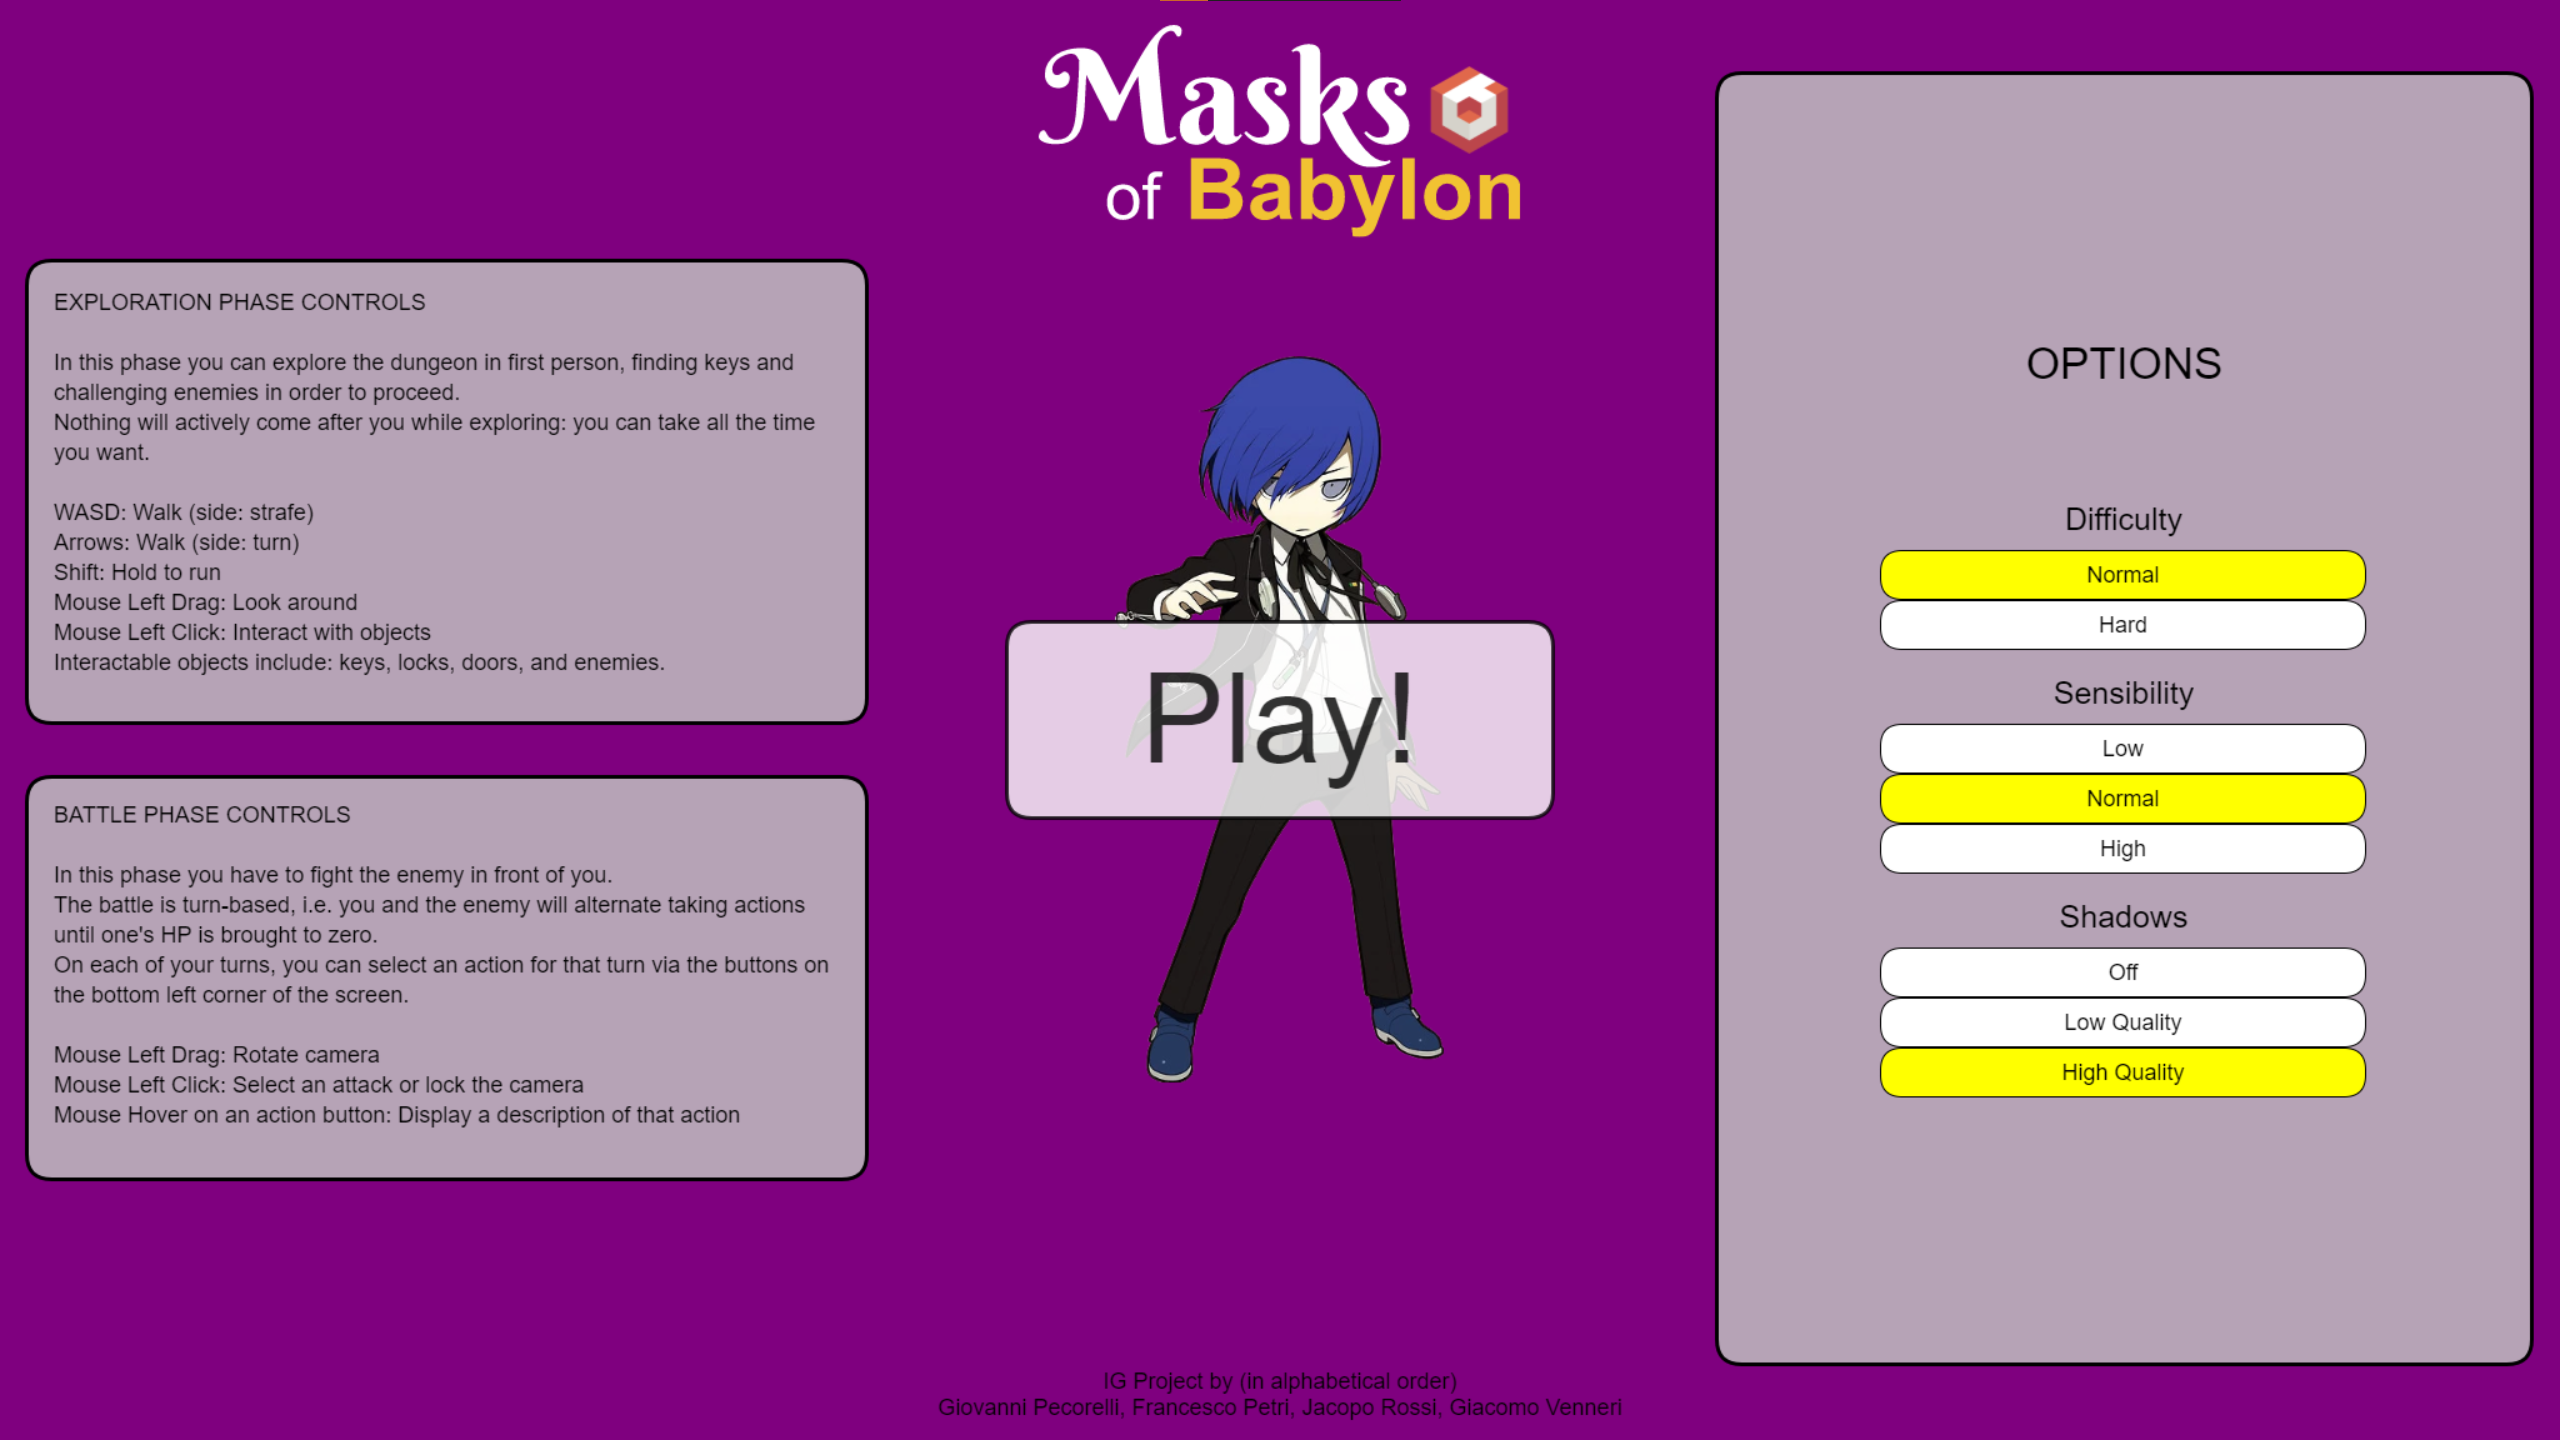
\includegraphics[width=0.9\textwidth]{images/ch2/main-menu.png}
    \caption{Main menu screen}
    \label{fig:main-menu}
\end{figure}

\section{Exploration Phase}

\subsection{Introduction and controls}
\label{sub:exploration-controls}

In this mode the dungeon is shown in a first-person view. The user can move and look around in multiple ways:

\begin{itemize}
    \item \textbf{WASD keys:} Move forward, left, backward and/or right with respect to where the camera is looking.
    \item \textbf{Arrow keys:} \textit{Up} and \textit{Down} move forward or backward, while \textit{Left} and \textit{Right} allow the user to turn around in their respective direction.
    \item \textbf{Mouse:} \textit{Hold the left button and move the mouse} to look around.
    \item \textbf{Shift:} Hold this key while moving with WASD or Arrows to walk faster.
\end{itemize}

Therefore the player can choose their preferred control scheme: moving with WASD and turning with the mouse, or using the arrows to do both at once but sacrificing some freedom.

\subsection{Interacting with objects}

Several interactable objects can be found throughout the play environment. Each of them can be interacted with by getting close to it and clicking on it with the left mouse button.



The following is a list of all interactable objects found in the project:

\begin{itemize}
    \item \textbf{Keys.} Click on a key to pick it up and carry it. The key can be used later to open a lock of the same color.
    \item \textbf{Locks.} These devices are always mounted on gates that block the way forward. If the user clicks on a lock while holding a key of the same color, the lock opens and the obstacle is removed. Otherwise, nothing happens.
    \item \textbf{Doors.} These objects can be used to move between the several areas the dungeon is composed of. Click on a door to go to the area it connects to.
    \item \textbf{Enemies.} Click on an enemy to enter the \textit{Battle Phase} and fight it. Enemies block the way until they are defeated.
\end{itemize}

These interactive objects can also be identified because the cursor changes from the default arrow to a pointing hand when hovering on one of them while the player is close enough to interact with it. \textit{However, because the \texttt{BABYLON.ActionManager} object, which we used to implement this behavior, offers events for the pointer entering or exiting a mesh but not for the pointer moving inside a mesh without entering or leaving, the cursor will not change if the user approaches the object from afar while keeping the cursor on it. The cursor will change as normal if the user then moves the cursor away from the interactive object and then back on it.}

\subsection{The story screen}

The very first time the user enters the dungeon after starting the game, a simple screen explaining the premise described above will be shown. The user only needs to read it and click OK to start playing.

\section{Battle Phase}

In this mode the player can fight one enemy in a turn-based battle, i.e. the two characters alternate taking actions to attack one another or to mitigate enemy attacks. The enemy won't attack during the player's turn no matter how much time the user takes to think, and neither character can act more than once before the other gets to take their turn.

The scene is shown in a side-view with the player character on the left and the enemy on the right, but the user can orbit the camera freely to explore a variety of third-person perspectives. UI elements in the corners of the screen show the amount of Health Points (HP) of each character.

The goal of a battle is to defeat the enemy character by reducing its HP to zero with attacks while avoiding that the player character's own HP fall to zero under the enemy's strikes.

\subsection{Battle actions}

During their turn, the user can select one action to take by clicking one of the four buttons that appear in the lower left area of the screen. If the user hovers on one of the buttons without clicking, they can read a short description of that action in the text box below.

Each action causes one or more animations and/or light effects to play and has some effect on the state of the battle.

The actions available to the player are the following:

\begin{itemize}
    \item \textbf{Attack.} The player character performs a simple slashing animation with his sword and causes the enemy to recoil because of the hit. The enemy takes a little damage to their HP.
    \item \textbf{Charge.} The player character transitions to a defensive pose, and then transitions back to their idle pose at the start of the next turn. This action causes the player to turn on their \textit{charge state}, which is needed to perform other actions, and halve any damage taken during that turn.
    \item \textbf{Fireball.} The player character performs a more elaborate animation in which he throws a fireball at the enemy, causing them to recoil and take higher damage to their HP. The player needs to have their \textit{charge state} on to perform this action, and executing it will turn it off again.
    \item \textbf{Prayer.} The player character performs an animation that represents him casting a healing spell and  recovers some HP, but he needs to have his \textit{charge state} on to perform this action, and executing it will turn it off again.
\end{itemize}

\subsection{The enemy turn}

Each enemy has two actions available to them: a normal attack and a stronger special attack. The enemy chooses an action at random on each of their turns, but the probability of choosing one or the other is influenced by the last action taken by the user: if the player used \textit{Fireball}, a strong attack, the enemy is more likely to retaliate with their own special attack; conversely, if the player used a non-offensive action like \textit{Charge} or \textit{Prayer}, the enemy will be more likely to use the normal attack.\\
Thus the user can also consider the most likely enemy response when planning their next move.

\subsection{Camera control}

At any time during the battle, the user can hold the left mouse button over the battle scene and move the cursor to orbit the camera around the arena.

A button on the bottom right corner of the screen allows the user to lock or unlock the camera: while it is locked, it returns to the default side view and cannot be moved this way until it is unlocked again.

\subsection{The victory screen}

This is a simple UI that appears when the player defeats the enemy by reducing its HP to zero.

Its purpose is to inform the player of the victory, and it includes a button that the user can click to proceed in the game.

\subsection{The game over screen}

This is a simple UI that appears when the player is defeated by the enemy to inform the user of the unfortunate event.

The user can click one of three buttons to decide what to do next:

\begin{itemize}
    \item \textbf{Retry the fight.} Restarts the current battle from the beginning.
    \item \textbf{Skip this battle.} Allows the player to skip the current battle as though they had won, in order to let any user see all the content in the project regardless of their expertise in turn-based RPG battles.
    \item \textbf{Quit to main menu.} Lets the user return to the main menu. All progress made through the dungeon will be lost.
\end{itemize}

\section{Ending scene}

Once the user defeats the boss of the dungeon, a simple scene is displayed to show the player character finally recovering the artifact he is looking for, and to inform the user they have completed the game.

The only interaction possible in this scene is a limited orbiting of the camera which works like in the battle scene, and a button in the lower right corner that lets the user return to the main menu.